% 1987 年全国卷文科第十八题：三棱锥 P-ABC 与公垂线 ED
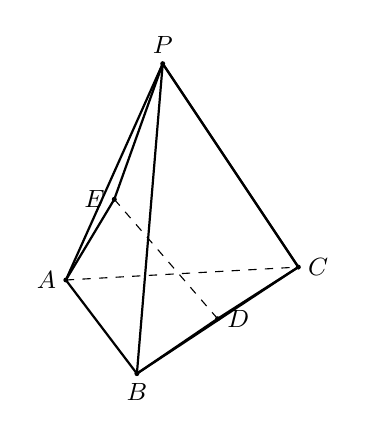
\begin{tikzpicture}[scale=0.82,>=stealth,font=\small]
  \coordinate (P) at (1.6,3.8);
  \coordinate (A) at (0.1,0.45);
  \coordinate (B) at (1.2,-1.0);
  \coordinate (C) at (3.7,0.65);
  \coordinate (E) at (0.85,1.7);
  \coordinate (D) at (2.45,-0.15);
  \draw[thick] (P)--(A)--(B)--(C)--cycle;
  \draw[thick] (P)--(B) (P)--(C);
  \draw[dashed] (A)--(C);
  \draw[dashed] (E)--(D);
  \draw[thick] (P)--(E) (E)--(A);
  \draw[thick] (B)--(D)--(C);
  \fill (P) circle (1.1pt) node[above] {$P$};
  \fill (A) circle (1.1pt) node[left] {$A$};
  \fill (B) circle (1.1pt) node[below] {$B$};
  \fill (C) circle (1.1pt) node[right] {$C$};
  \fill (E) circle (1.1pt) node[left] {$E$};
  \fill (D) circle (1.1pt) node[right] {$D$};
\end{tikzpicture}
